\documentclass[10pt,xcolor=table, aspectratio=1610]{beamer}
% \special{dvipdfmx:config z 0}
\usetheme[progressbar=frametitle]{metropolis}
\usepackage[export]{adjustbox}
\usepackage{appendixnumberbeamer}
\usepackage{booktabs}
\usepackage{ellipsis}
\usepackage{hhline}
\usepackage{textgreek}
\usepackage{url}
\usepackage[outputdir=out]{minted}
\usepackage{csquotes}

\def\UrlBreaks{\do\/\do-}

\usepackage{caption}
\captionsetup{justification=raggedright,
              singlelinecheck=off,
              font=scriptsize,
              labelfont=scriptsize}
\setlength{\abovecaptionskip}{2pt}
\setlength{\belowcaptionskip}{0pt}

\setbeamertemplate{footline}{
  \begin{beamercolorbox}{footer nav}
    \vskip 2pt \insertnavigation{\paperwidth} \vskip 2pt
  \end{beamercolorbox}
}


\title{Smart TASEP}
\subtitle{Deep Q-Learning in Intelligent Matter Simulations}
\date{\today}
\author{Jonas Märtens}
\institute{LMU Munich}

\begin{document}
\maketitle

\section{Introduction}
\begin{frame}{Overview}
    \begin{columns}
      \column{0.5\textwidth}
      \begin{block}{Smart TASEP: Deep Q-Learning in Intelligent Matter Simulations}
      \begin{itemize}
        \item TASEP: Totally Asymmetric Simple Exclusion Process
        \item Smart TASEP: TASEP with intelligent agents \\
              $\rightarrow$ Intelligent Matter Simulations
        \item Deep Q-Learning: Reinforcement Learning with Neural Networks
      \end{itemize}
      \end{block}
      \column{0.5\textwidth}
      \begin{figure}
        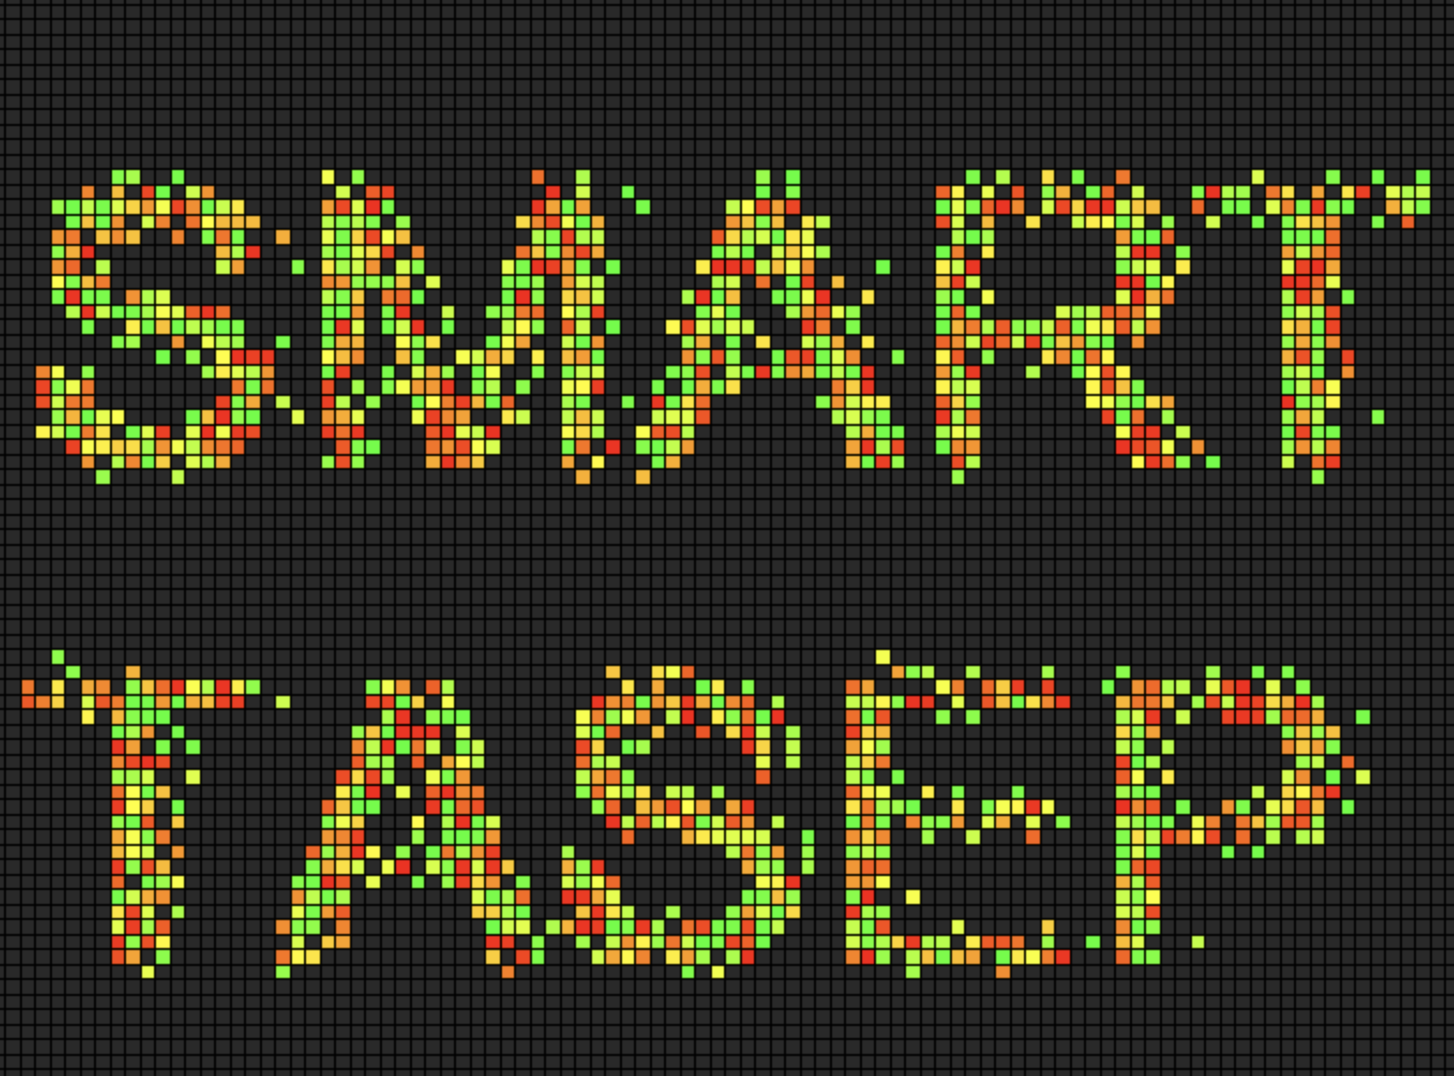
\includegraphics[width=\textwidth]{img/smarttasep.png}
      \end{figure}
    \end{columns}
\end{frame}


\begin{frame}{TASEP}
    \begin{columns}
      \column{0.5\textwidth}
      \begin{block}{TASEP: \alert<4>{Totally Asymmetric} \alert<3>{Simple} \alert<2>{Exclusion} \alert<1>{Process}}
      \begin{itemize}
        \item<1-> Stochastic Process on a grid lattice
        \item<2-> Exclusion: Only one particle per site
        \item<3-> Simple: Jumps only one cell far 
        \item<4-> Totally Asymmetric: $p=1,q=0$
      \end{itemize}
      \onslide<5->{
      Possible with either
      \begin{itemize}
        \item Periodic boundary conditions
        \item Open boundary conditions
      \end{itemize}
      }
      \end{block}
      \column{0.5\textwidth}
      \begin{figure}
        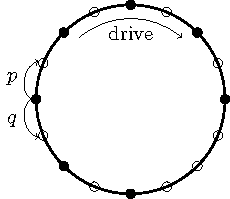
\includegraphics[width=0.7\textwidth]{../Thesis/img/model/out/tasep_a.pdf}
        \caption*{ASEP with periodic boundary conditions}
      \end{figure}
      \begin{figure}
        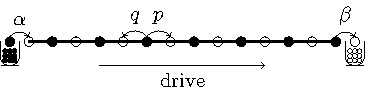
\includegraphics[width=\textwidth]{../Thesis/img/model/out/tasep_b.pdf}
        \caption*{ASEP with open boundary conditions}
      \end{figure}
    \end{columns}
\end{frame}

\begin{frame}{Modifications}
    \begin{columns}
      \column{0.5\textwidth}
      Two modifications (before smarticles)
      \begin{block}{2D (T)ASEP}
        \begin{itemize}
          \item Symmetric in one direction and totally asymmetric in the other
          \item<2-> Directed flow with multiple lanes
          \item<2-> compare traffic flow, kinesin transport
          \item<2-> motivates transport optimization
        \end{itemize}
      \end{block}
      \onslide<3->{
      \begin{block}{Speeds}
        \begin{itemize}
          \item Each particle has a speed
          \item Speed is probability to jump
          \item Drawn from a distribution
          \item If different, jams
        \end{itemize}
      \end{block}
      }
      \column{0.4\textwidth}
      \begin{figure}
        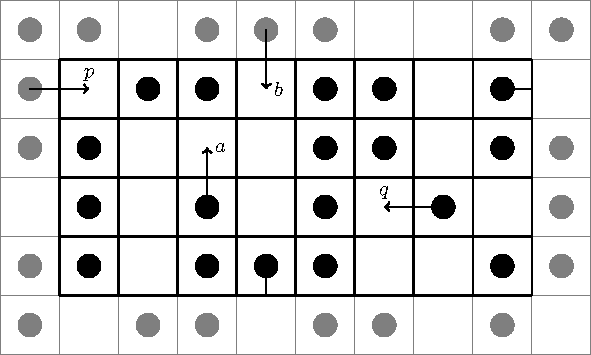
\includegraphics[width=\textwidth]{../Thesis/img/model/out/tasep_2d_nodrive.pdf}
        \caption*{2D ASEP}
      \end{figure}
      \vskip -1em
      \onslide<2->{
      \begin{figure}
        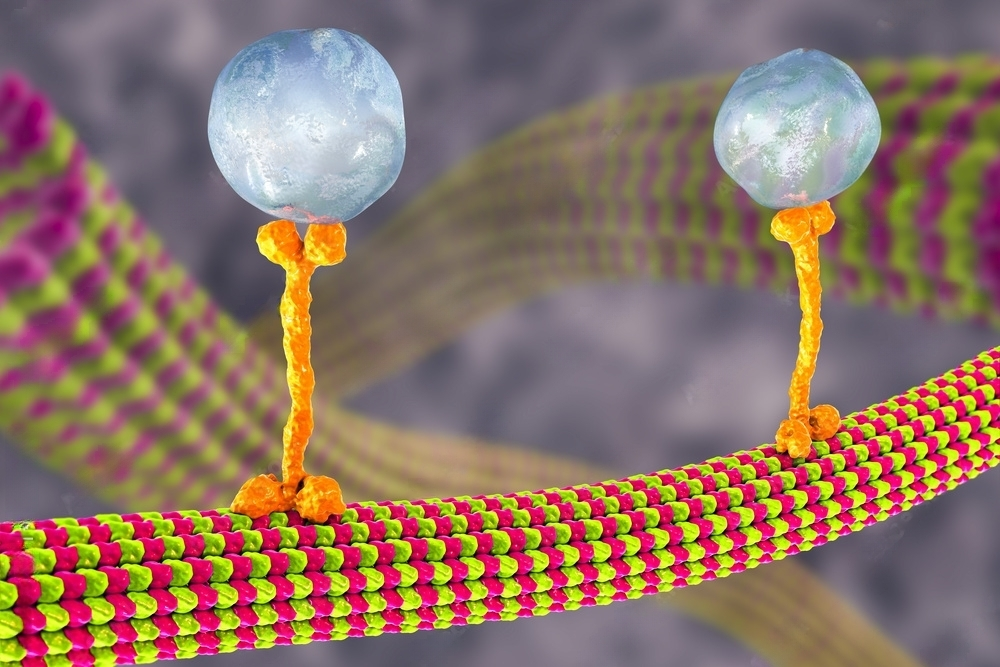
\includegraphics[width=\textwidth]{img/kinesin.jpeg}
        \caption*{Intracellular transport}
      \end{figure}
      }
    \end{columns}
\end{frame}

\section{Make it Smart!}
\begin{frame}{Smart TASEP}
    \begin{columns}
      \column{0.5\textwidth}
      \begin{block}{Smart TASEP: TASEP with intelligent agents}
      \begin{itemize}
        \item have a goal (e.g. optimize transport)
        \item sense the environment
        \item act according to the goal and the environment
        \item learn from the environment themselves
      \end{itemize}
      $\rightarrow$ Intelligent Matter Simulation \\
      $\rightarrow$ Reinforcement Learning - reward based
      \end{block}
      \column{0.5\textwidth}
      \begin{figure}
        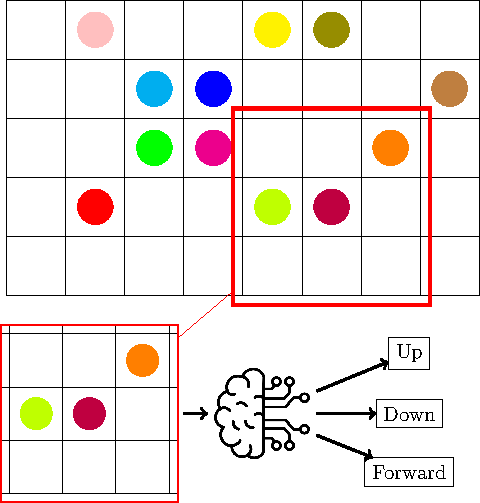
\includegraphics[width=\textwidth]{img/out/agents.pdf}
      \end{figure}
    \end{columns}
\end{frame}

\section{Deep Q-Learning}
\begin{frame}{Deep Q-Learning: Overview}
    \begin{columns}
      \column{0.6\textwidth}
      \begin{block}{Deep Q-Learning Algorithm}
        \begin{itemize}
          \item Reinforcement learning with deep neural networks
          \item Model-free: No knowledge of the environment
          \item Q-Learning: Value-based method
          \item Off-policy: Learns from old experiences
        \end{itemize}
      \end{block}
      \column{0.4\textwidth}
      \begin{figure}
        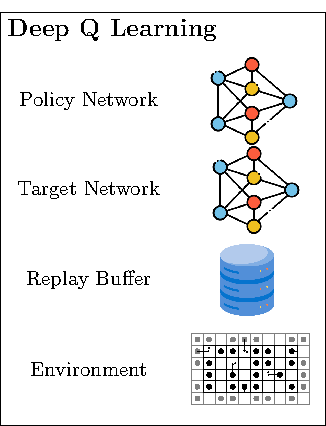
\includegraphics[width=\textwidth]{img/out/dql.pdf}
      \end{figure}
    \end{columns}
\end{frame}


\begin{frame}{Deep Q-Learning: The policy}
  \vskip -1em
    \begin{figure}
      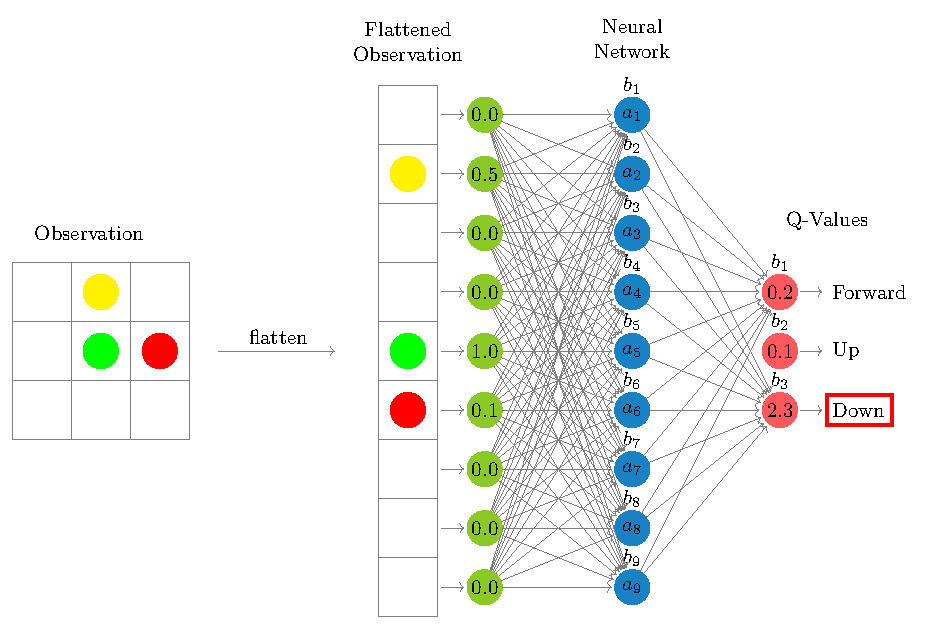
\includegraphics[width=0.9\textwidth]{img/out/policy_net.pdf}
    \end{figure}
\end{frame}


\begin{frame}{Deep Q-Learning: Optimization}
    \begin{columns}
      \column{0.55\textwidth}
      \begin{block}{How does the network learn?}
        \begin{itemize}
          \item Neural Network $\rightarrow$ backpropagation on loss
          \item Problem: no target value for Q-Learning
          \item Solution: Use current best guess as target: \\
                $y = r + \gamma \max_{a'} \hat{Q}(s', a')$
          \item Target network with soft updates to stabilize learning
          \item Use gradients for AdamW optimizer
          \item Replay buffer
                \begin{itemize}
                  \item Sample efficiency
                  \item Break correlation
                \end{itemize}
        \end{itemize}
      \end{block}
      \column{0.45\textwidth}
      \begin{figure}
        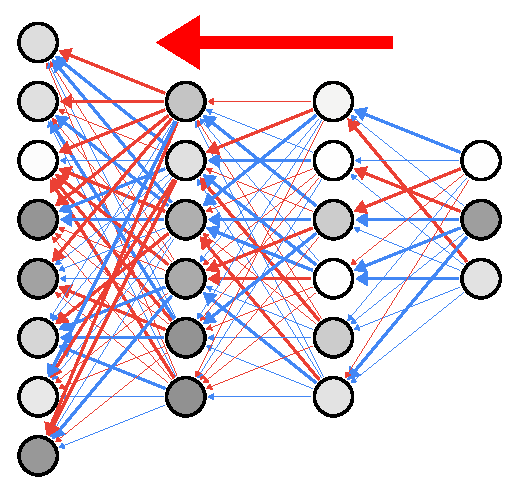
\includegraphics[width=\textwidth]{img/out/backprop.pdf}
      \end{figure}
    \end{columns}
\end{frame}

\section{Implementation}
\begin{frame}{The \texttt{smarttasep} package}
    \begin{columns}
      \column{0.4\textwidth}
      \begin{block}{Features}
        \begin{itemize}
          \item Easy installation with \texttt{pip}
          \item Fully Customizable
          \begin{itemize}
            \item Environment size
            \item Reward function
            \item Network architecture
            \item Hyperparameters
            \item Training parameters
            \item Algorithm choices
          \end{itemize}
          \item Real-time visualization
          \item Interactive evaluation
          \item Management of experiments
        \end{itemize}
      \end{block}
      \column{0.6\textwidth}
      \begin{block}{\texttt{smarttasep} components}
        \begin{itemize}
          \item \texttt{smarttasep.GridEnv}: The 2D (T)ASEP environment
          \item \texttt{smarttasep.DQN}: The neural network
          \item \texttt{torchrl.ReplayBuffer}: Efficient, tensor-based replay buffer
          \item \texttt{smarttasep.Trainer}: Wrapper class for training, simulation and experiment management
          \item \texttt{smarttasep.Playground}: Real-time interactive evaluation of trained agents
          \item \texttt{smarttasep.EnvParams, smarttasep.Hyperparams}: Configuration classes
        \end{itemize}    
      \end{block}
    \end{columns}
\end{frame}

\begin{frame}{Hyperparameter Optimization}
  For each experiment, the Hyperparameters should be optimized. 
    \begin{block}{Parameters}
      \begin{itemize}
        \item \textbf{Learning rate} of the AdamW optimizer.
        \item \textbf{Discount factor} $\gamma$.
        \item \textbf{Replay buffer size}.
        \item \textbf{Batch size} for training.
        \item \textbf{Target network update rate} $\tau$.
        \item \textbf{Exploration-exploitation tradeoff} via the decay constant $\eta$ of the exploration rate $\epsilon(t)=\epsilon_{\text{end}} + (\epsilon_{\text{start}} - \epsilon_{\text{end}}) e^{-n_{\text{steps}}/\eta}$.
        \item \textbf{Neural network architecture} (number of hidden layers and neurons per layer).
        \item \textbf{Activation function} of the neural network.
    \end{itemize}
    \end{block}
\end{frame}

\begin{frame}{Hyperparameter Optimization: Example}
  \begin{figure}
    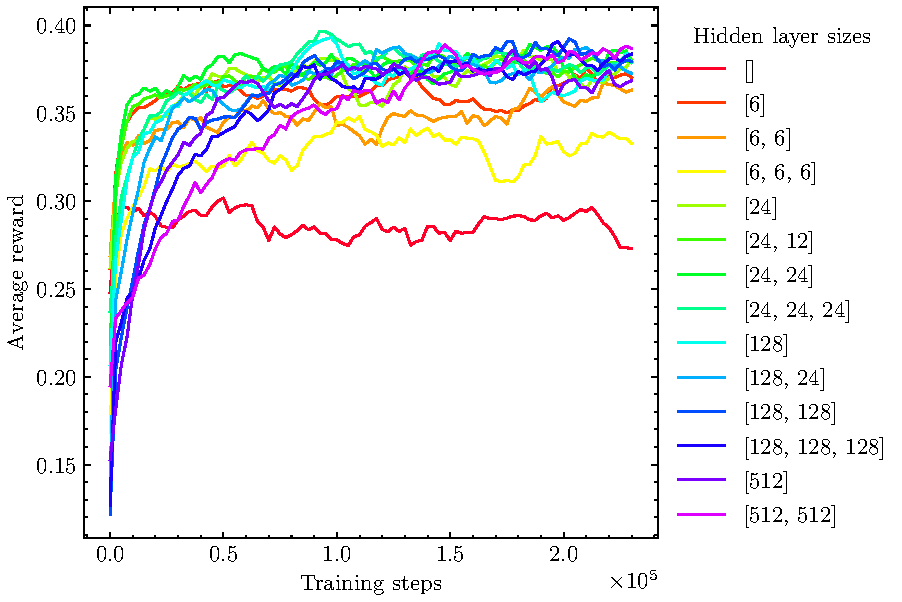
\includegraphics[width=0.7\textwidth]{img/hyperparam_optim_hidden_layer_sizes.pdf}
    \caption*{\hspace{2cm} Example of a hyperparameter optimization for the hidden layer sizes.}
  \end{figure}
\end{frame}

\section[Results]{Results}
\begin{frame}{Overview of Experiments}
  \begin{block}{Goals}
    \begin{itemize}
      \item Current optimization
      \item General insights into intelligent matter simulations  
    \end{itemize}
  \end{block}
  \begin{block}{Experiments}
  \begin{enumerate}
    \item \textbf{Baseline}: Classical 2D TASEP with speeds
    \item \textbf{Naive current optimization}: Hard-coded agents
    \item \textbf{Smart TASEP}: Deep Q-Learning agents with slightly different goals
    \begin{itemize}
      \item \textbf{Simple reward}: Go forward
      \item \textbf{Complex reward}: Go forward while forming lanes
    \end{itemize}
  \end{enumerate}
  \end{block}
\end{frame}

\begin{frame}{Results: Baseline}
  \begin{columns}
    \column{0.35\textwidth}
    \begin{block}{Setup}
      \begin{itemize}
        \item Classical 2D TASEP
        \item Periodic boundary conditions
        \item Checkerboard configuration
        \item<2-> Normally distributed speeds
        \item<3-> Waiting for steady state
        \item<4-> Measuring average current
        \item<4-> Consistent with theoretical value of 0.0625
      \end{itemize}
    \end{block}
    \column{0.6\textwidth}
    \begin{overprint}
    \onslide<2>\begin{figure}
      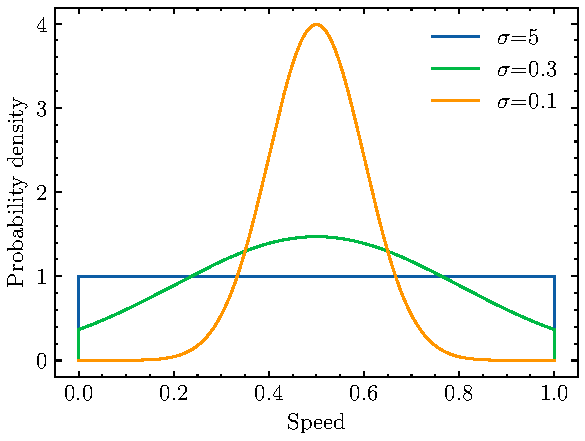
\includegraphics[width=0.65\textwidth]{../Thesis/img/results/truncated_normal.pdf}
      \caption*{\hspace{0.175\textwidth} Speeds of particles in the baseline experiment.}
    \end{figure}
    \onslide<3>\begin{figure}
      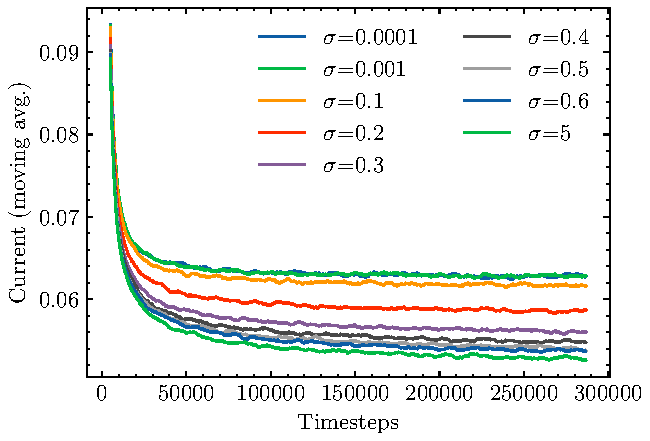
\includegraphics[width=\textwidth]{../Thesis/img/results/currents_fixed_sigma_128x32.pdf}
      \caption*{Reaching the steady state in a 128x32 system. \\ 800 runs and 5000 steps averaged.}
    \end{figure}
    \onslide<4->\begin{figure}
      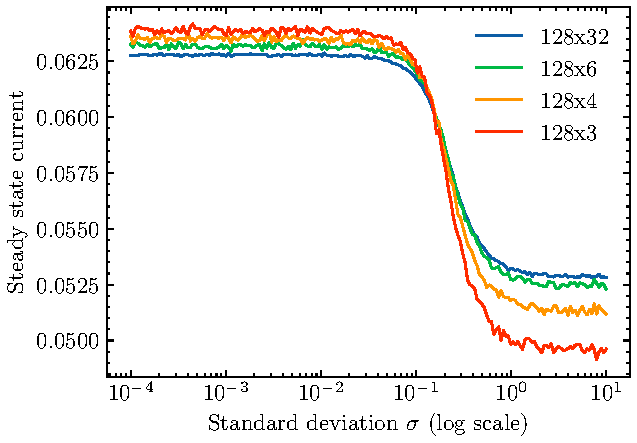
\includegraphics[width=\textwidth]{../Thesis/img/results/steady_state_current_sizes_log.pdf}
      \caption*{Steady state current as a function of $\sigma$ for different system sizes.\\800 runs and 150k steps averaged.}
    \end{figure}
    \end{overprint}
  \end{columns}
\end{frame}

\section[Naive Policy]{Results: Naive Optimization}
\begin{frame}{A Naive Policy}
  \begin{columns}
    \column{0.35\textwidth}
    \begin{block}{Just go forward?}
      \begin{itemize}
        \item $p_\text{fwd} = 1, p_\text{up/down} = 0$
        \item starting in checkerboard configuration
        \item no messy mixing
        \item bad for high $\sigma$
        \item optimum for low $\sigma$?
      \end{itemize}
    \end{block}
    \column{0.6\textwidth}
    \begin{figure}
      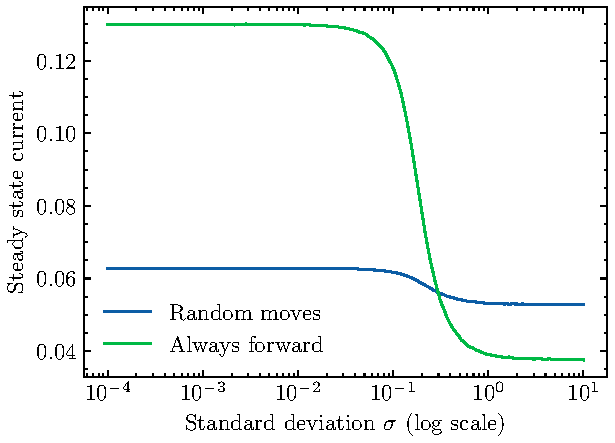
\includegraphics[width=\textwidth]{../Thesis/img/results/steady_state_current_both_log.pdf}
      \caption*{Naive policy}
    \end{figure}
  \end{columns}
\end{frame}

\section[Smarticles]{Results: Smarticles}

\begin{frame}{Smarticles: Uniform speed distribution}
  \begin{columns}
    \column{0.35\textwidth}
    \begin{block}{Simple reward components, $\sigma=10$}
      \begin{itemize}
        \item Positive reward for going forward
        \item Negative reward for occupied destination
        \item Zero reward for going up or down or staying
        \item Small negative reward for blocking others proportional to speed
      \end{itemize}
    \end{block}
    \column{0.65\textwidth}
    \begin{figure}
        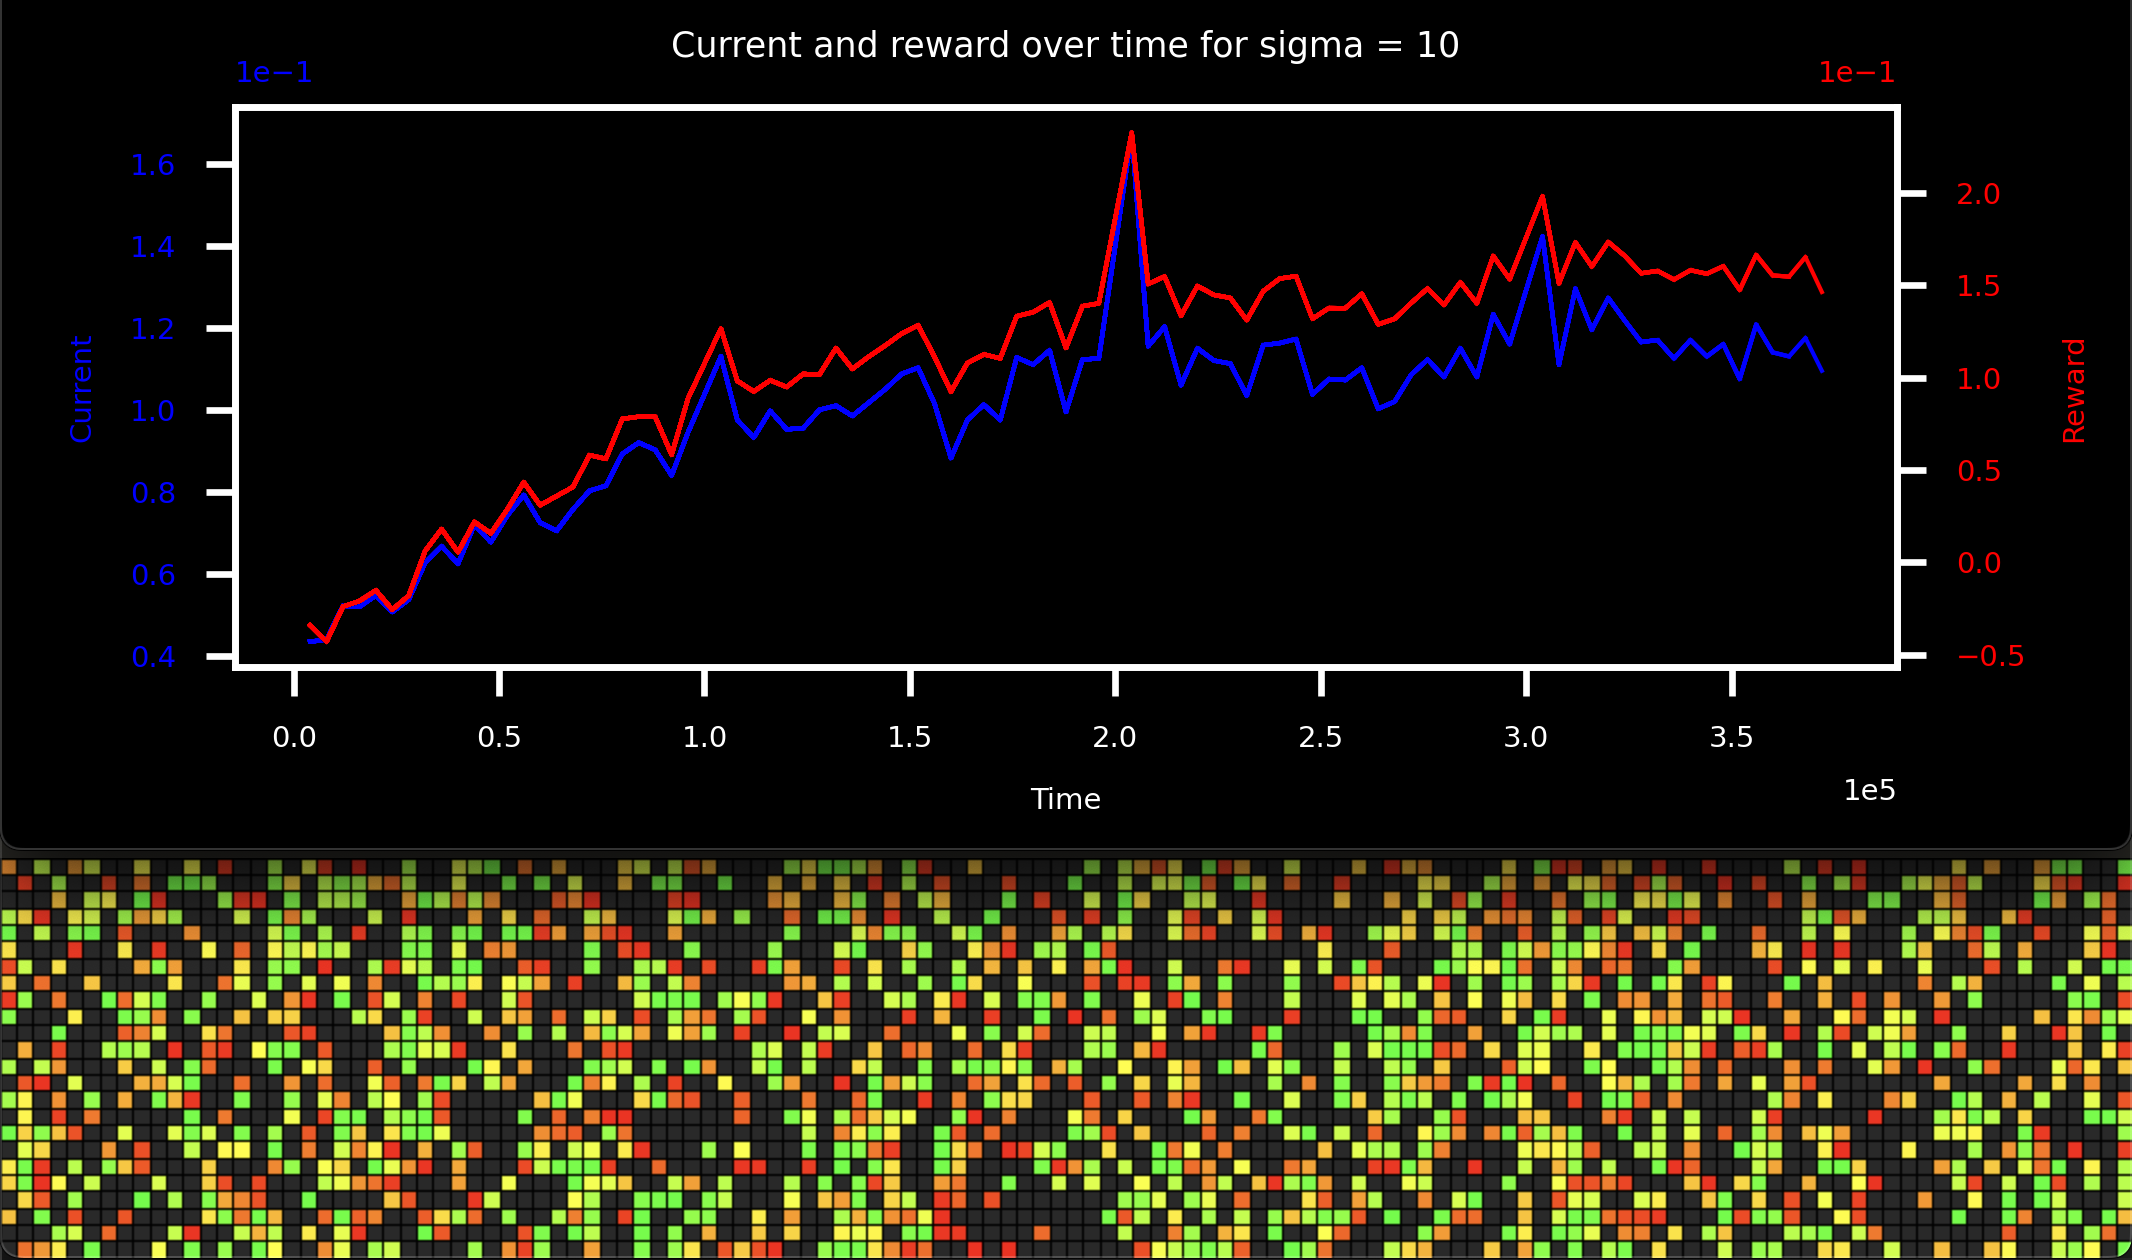
\includegraphics[width=\textwidth]{../Thesis/img/results/second_training_screenshot.png}
        \caption*{Screenshot of the second smarticle training}
      \end{figure}
  \end{columns}
\end{frame}

\begin{frame}{Smarticles: Uniform speed distribution}
  \begin{columns}
    \column{0.45\textwidth}
    \begin{block}{Resulting current}
      \begin{itemize}
        \item $\left\langle J \right\rangle \approx 0.117$
        \item $+125\%$ compared to baseline (0.052)
        \item Lower than with equal speeds
      \end{itemize}
    \end{block}
    \column{0.55\textwidth}
    \begin{figure}
        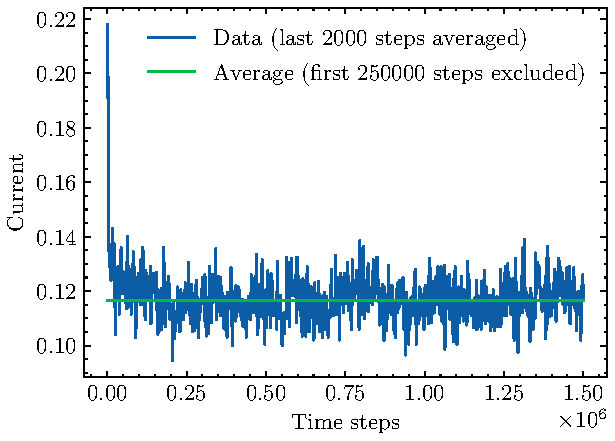
\includegraphics[width=\textwidth]{../Thesis/img/results/uniform_speeds.pdf}
        \caption*{Steady state current over time for the trained smarticles.}
      \end{figure}
  \end{columns}
\end{frame}

\begin{frame}{Smarticles: Model Analysis}
  What did the smarticles learn? (Playground video)
\end{frame}

\begin{frame}{Smarticles: Why Global Structures}
  \begin{columns}
    \column{0.5\textwidth}
    \begin{block}{Observation}
      \begin{itemize}
        \item So far, the system still looks messy
        \item Only individual behavior
        \item Compare highway: Fast lane and slow lane
        $\rightarrow$ Could be beneficial also in TASEP 
      \end{itemize}
    \end{block}
    \begin{block}{Potential}
      \begin{itemize}
        \item Less jamming
        \item Directed flow without dispersion
        \item Inhomogeneous density
      \end{itemize}
    \end{block}
    \column{0.5\textwidth}
    \begin{figure}
      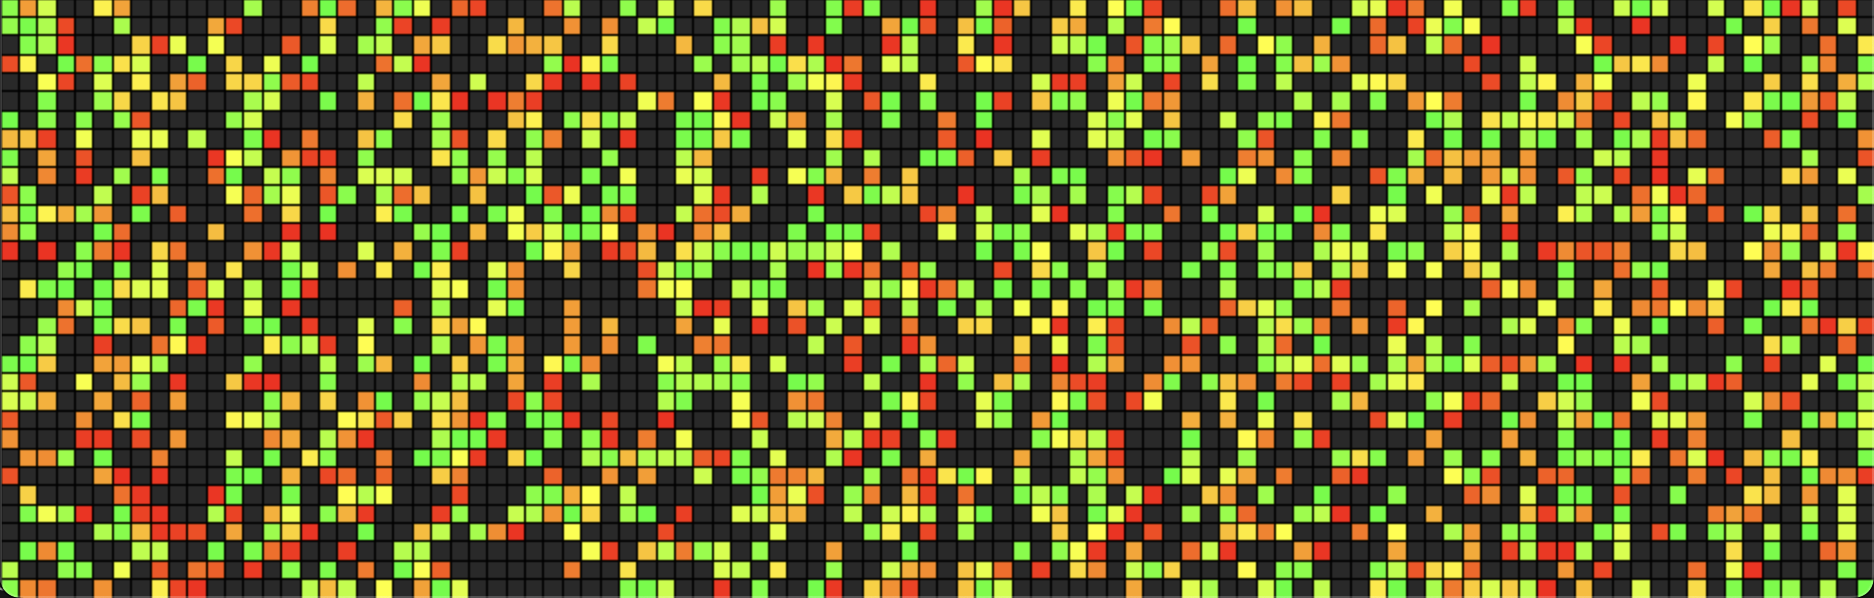
\includegraphics[width=\textwidth]{img/messy_tasep.png}
      \caption*{Screenshot of the simulation with the current policy}
    \end{figure}
    \begin{figure}
      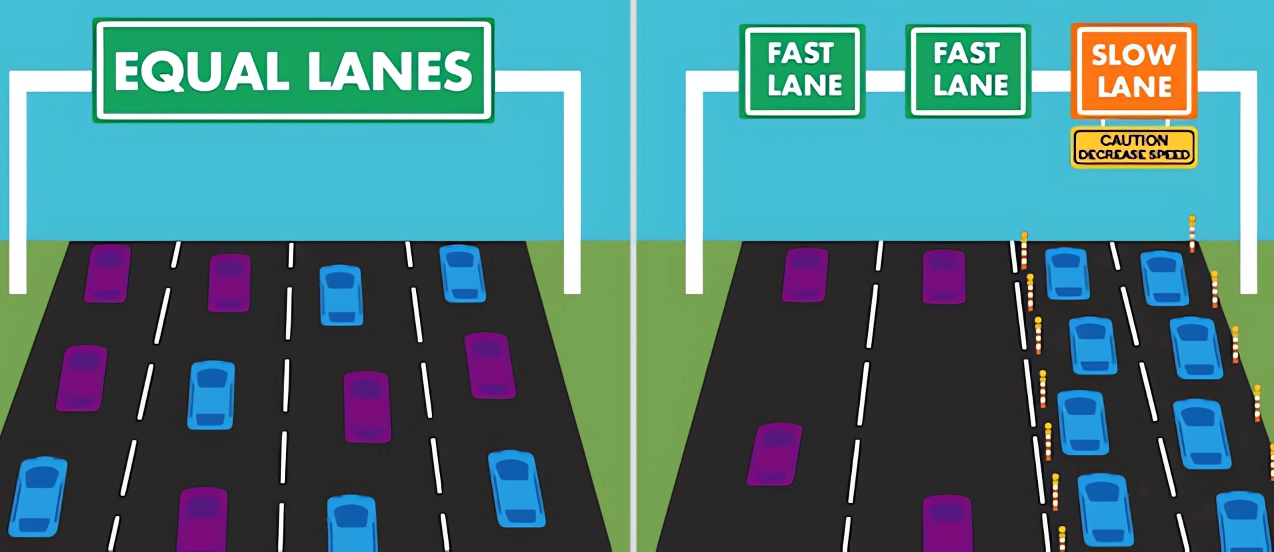
\includegraphics[width=\textwidth]{img/fast_lane_slow_lane.png}
      \caption*{Separating fast and slow lanes increases the mean velocity}
    \end{figure}
  \end{columns}
\end{frame}

\begin{frame}{Smarticles: Hard-coded Lanes}
  \textbf{Approach 1}: Hard code the lanes, supply smarticles with lane information\\
  \begin{equation*}
    \Delta y = 1-a\cdot\left(\frac{1+a}{a}\right)^v+a
  \end{equation*}
  \begin{figure}
    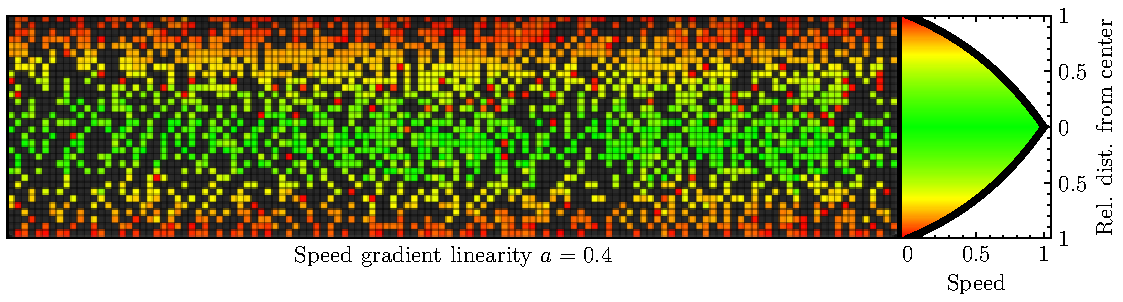
\includegraphics[width=\textwidth]{../Thesis/img/results/speed_gradient_0.4.pdf}
    \caption*{Learned smarticle behavior with the hard-coded lanes reward function (left), and the speed gradient mapping (right).}
  \end{figure}
\end{frame}

\begin{frame}{Smarticles: Hard-coded Lanes - Results}
  \begin{columns}
    \column{0.45\textwidth}
    \begin{block}{Resulting current}
      \begin{itemize}
        \item $\left\langle J \right\rangle \approx 0.134$
        \item $+157\%$ compared to baseline (0.052)
        \item $+15\%$ compared to previous policy (0.117)
        \item long time to reach steady state
      \end{itemize}
    \end{block}
    \column{0.55\textwidth}
    \begin{figure}
        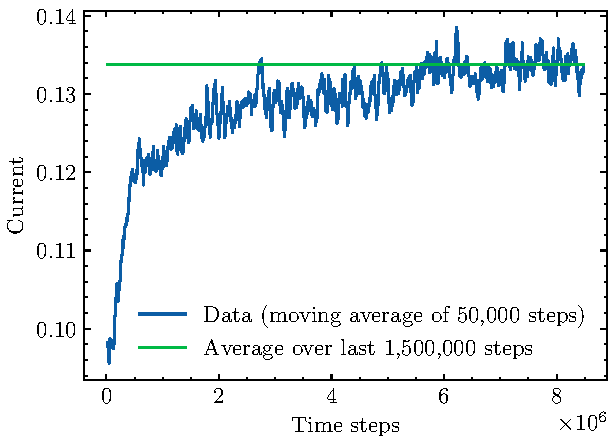
\includegraphics[width=\textwidth]{../Thesis/img/results/speed_grad_current.pdf}
        \caption*{Current over time for the trained smarticles.}
      \end{figure}
  \end{columns}
\end{frame}

\begin{frame}{Smarticles: Self-organized Lanes}
  \onslide<1->Absolute positioning for hard-coded lanes is not always possible.\\
  \onslide<2->
  \textbf{Approach 2}: Let the smarticles learn the lanes themselves from local \enquote{interactions}\\
  \begin{equation*}
    \text{V}(r, \Delta v) = \begin{cases}
      -0.125 \cdot r + 0.625 & \text{if } \Delta v < 0.5 \text{ and } 1.5 < r \le 5 \\
      -0.75 \cdot r^{-1.3} - 0.15 & \text{if } \Delta v \ge 0.5 \text{ and } r \le 3.5 \\
      0 & \text{otherwise}
  \end{cases}
  \end{equation*}
  \begin{block}{Modifications}
    \begin{enumerate}
      \item Binary speed distribution
      \item Different neural networks
    \end{enumerate}
  \end{block}
\end{frame}

\begin{frame}
  \begin{figure}
    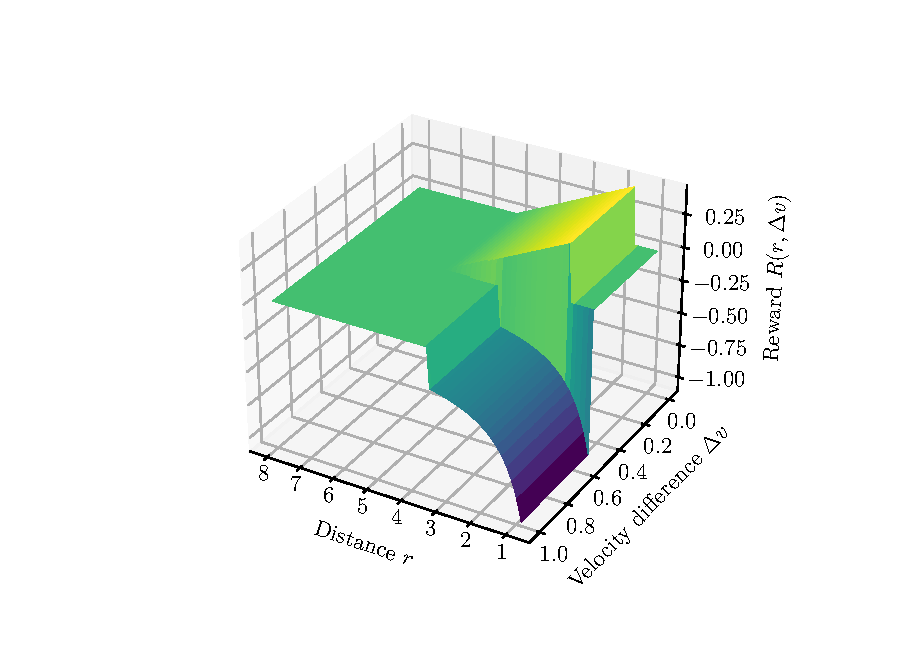
\includegraphics[width=0.6\textwidth]{../Thesis/img/results/lane_reward_func_3d_cropped.pdf}
    \caption*{\hspace{0.2\textwidth}Visual representation of the lane reward function / \enquote{potential}}
  \end{figure}
\end{frame}

\begin{frame}{Smarticles: Self-organized Lanes - Results}
  Let's see it in action! (lane formation video)
\end{frame}

\begin{frame}{Smarticles: Self-organized Lanes - Results}
  \begin{columns}
    \column{0.45\textwidth}
    \begin{block}{Resulting current}
      \begin{itemize}
        \item $\left\langle J \right\rangle \approx 0.112$
        \item baseline $J=0.4\cdot(1-0.4)\cdot0.6\cdot0.5=0.072$
        \item $+56\%$ compared to baseline
        \item lower than previous policies
        \item steady state reached quicker
        \item fluctuations seem higher than they are
        \item proof of concept, room for improvement
      \end{itemize}
    \end{block}
    \column{0.55\textwidth}
    \begin{figure}
        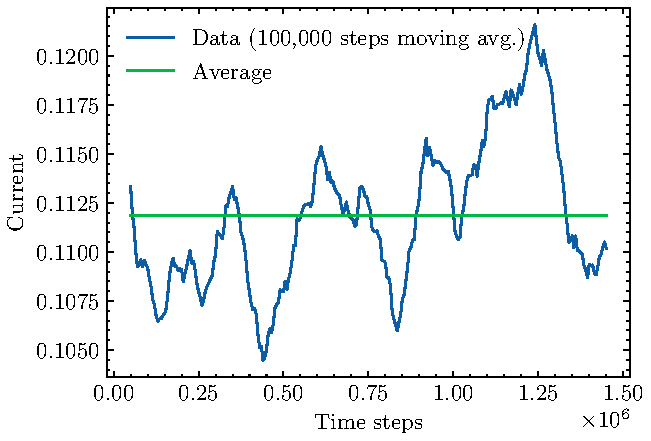
\includegraphics[width=\textwidth]{../Thesis/img/results/lanes_current.pdf}
        \caption*{Current over time for the trained smarticles.}
      \end{figure}
  \end{columns}
\end{frame}

\section{Conclusion and Outlook}
\begin{frame}{Conclusion and Outlook}
  \begin{columns}
    \column{0.5\textwidth}
    \begin{block}{Achievements and Insights}
      \begin{itemize}
        \item Baseline: Theory and simulation match
        \item Established framework for intelligent matter simulations with interacting agents
        \item Intelligent matter in form of smarticles dramatically increases the current
        \item Large-scale structures and collective behavior emerge from local \enquote{interactions}
      \end{itemize}
    \end{block}
    \column{0.5\textwidth}
    \begin{block}{Future Research}
      \begin{itemize}
        \item Modular \texttt{smarttasep} package for easy experimentation
        \item Generalize results:
        \begin{itemize}
          \item Structure formation with more than two particle types
          \item Different cluster densities for different speeds
          \item Reduce the gap between the lanes
        \end{itemize}
        \item Try different strategies other than lane formation
        \item Generalize results to more complex systems (e.g. higher dimensions, continuous space)
      \end{itemize}
    \end{block}
  \end{columns}
\end{frame}

\appendix
\section*{Backup Slides}

\begin{frame}{Smarticles: Equal speeds}
  \begin{columns}
    \column{0.35\textwidth}
    \begin{block}{Simple reward}
      \begin{itemize}
        \item Positive reward for going forward
        \item Negative reward for occupied destination
        \item Zero reward for going up or down or staying
        \item Small negative reward for blocking others
      \end{itemize}
    \end{block}

    \column{0.65\textwidth}
      \begin{figure}
        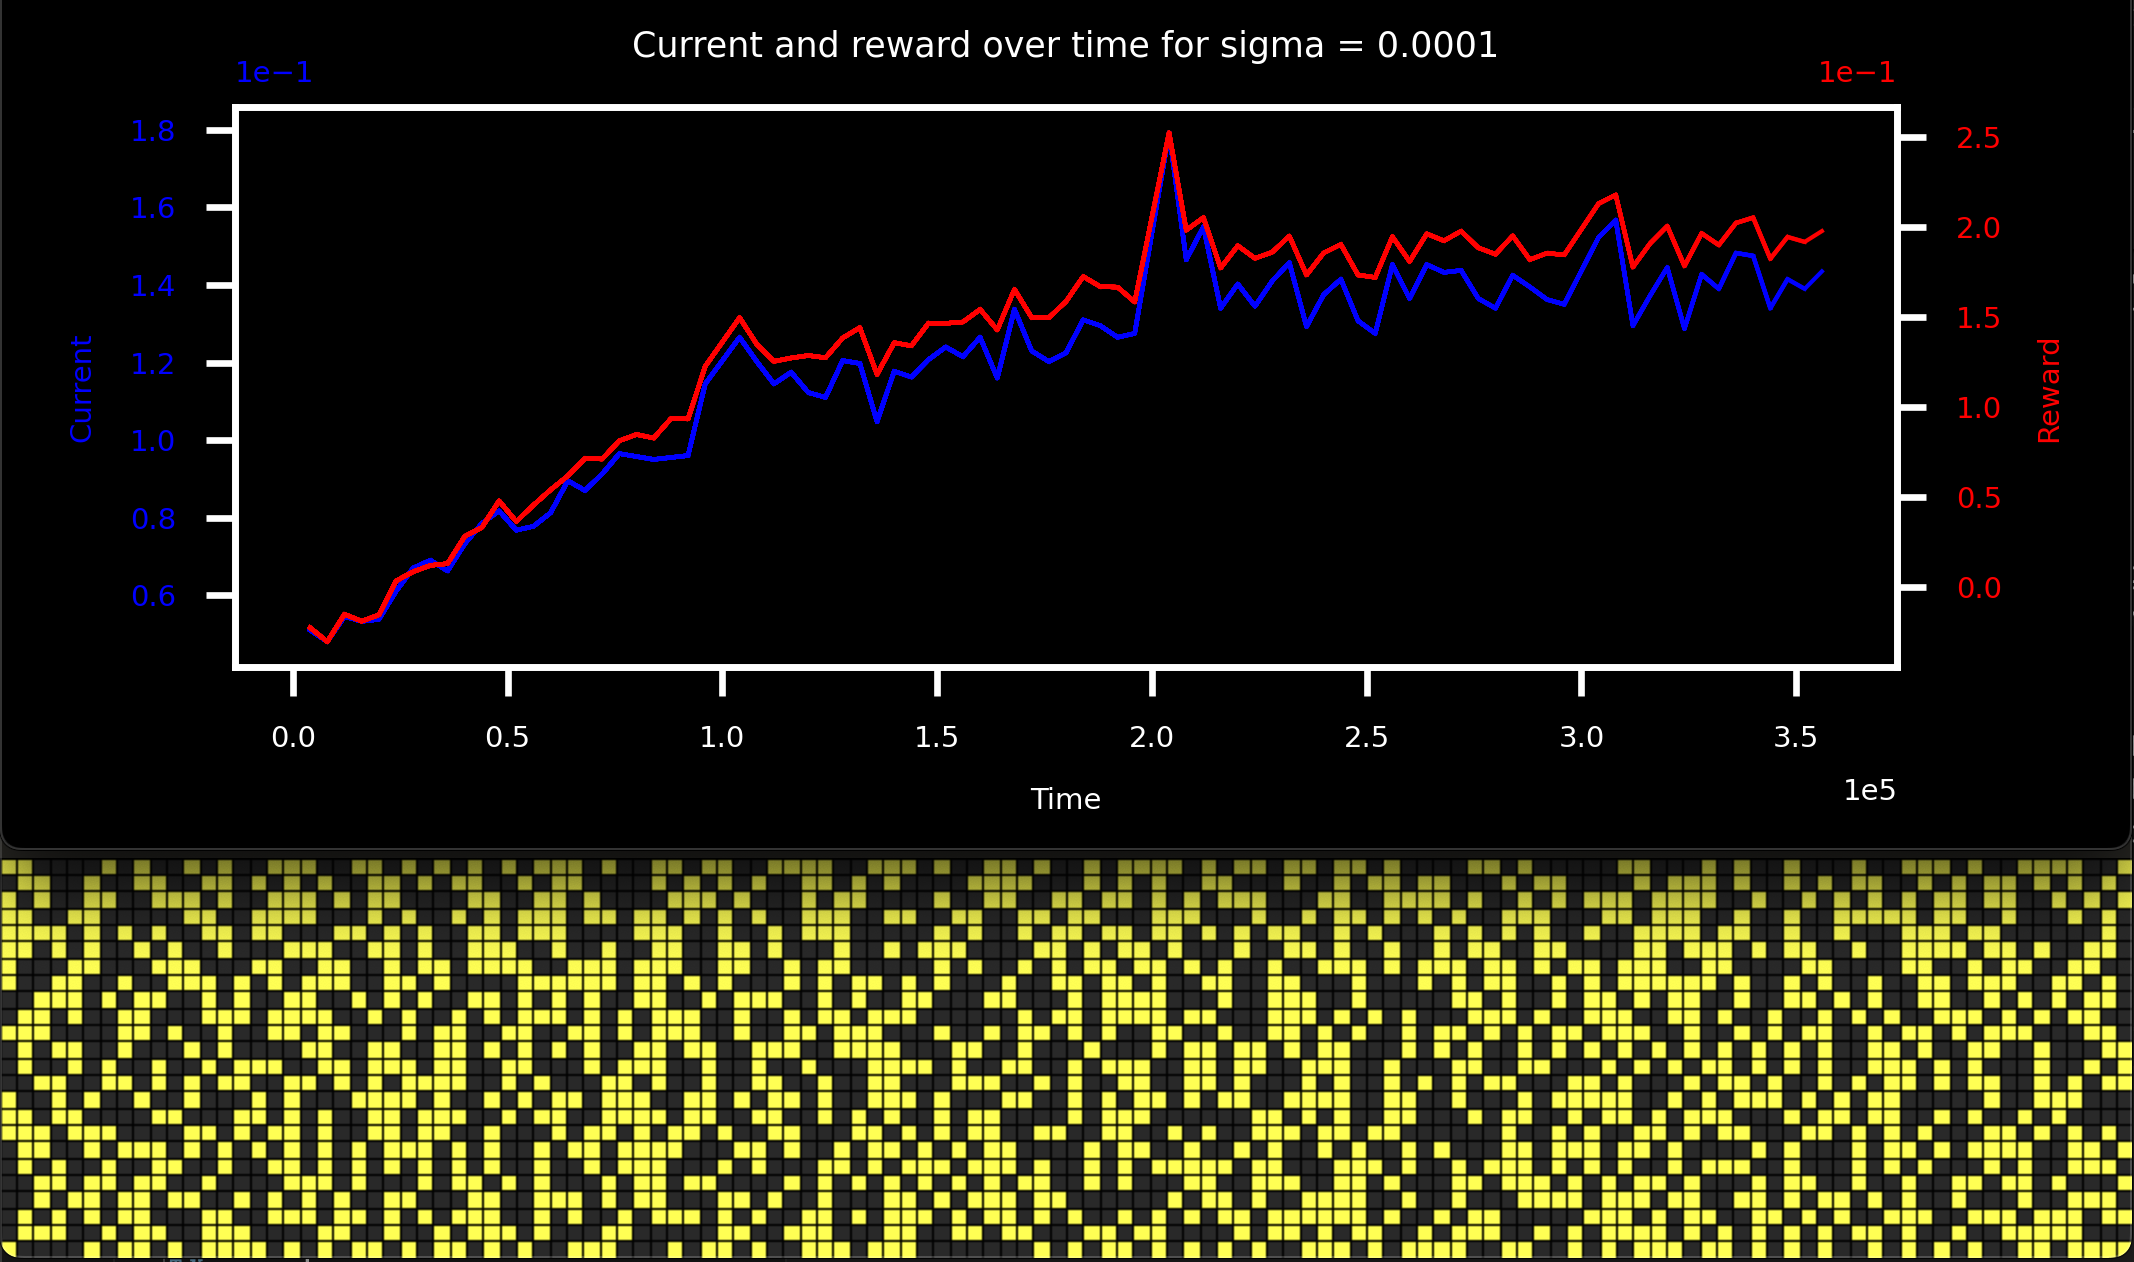
\includegraphics[width=\textwidth]{../Thesis/img/results/first_training_screenshot.png}
        \caption*{Screenshot of the first smarticle training}
      \end{figure}
      
  \end{columns}

\end{frame}

\begin{frame}{Smarticles: Equal speeds}
  \begin{columns}
    \column{0.45\textwidth}
    \begin{block}{Resulting current}
      \begin{itemize}
        \item $\left\langle J \right\rangle \approx 0.152$
        \item $+143\%$ compared to baseline (0.0625)
        \item $+22\%$ compared to naive policy (0.125)
      \end{itemize}
    \end{block}
    \column{0.55\textwidth}
    \begin{figure}
        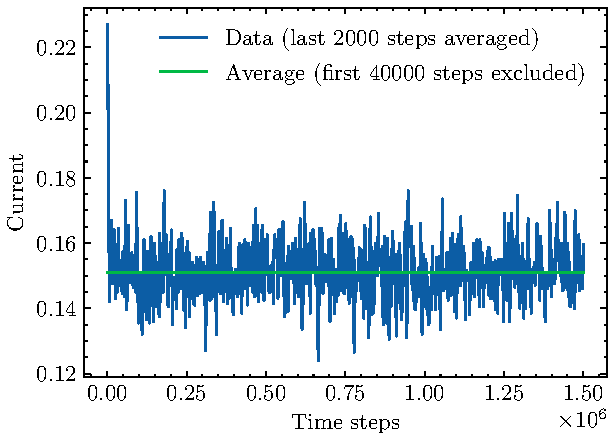
\includegraphics[width=\textwidth]{../Thesis/img/results/equal_speeds.pdf}
        \caption*{Steady state current over time for the trained smarticles.}
      \end{figure}
  \end{columns}
\end{frame}

\begin{frame}{The \texttt{smarttasep} package: Examples}
  Let's have a look at some examples! (show usage videos)
\end{frame}

\begin{frame}{Results: Theory}
  \begin{columns}
    \column{0.35\textwidth}
    \begin{block}{Conditions for a forward move}
      \begin{enumerate}
        \item randomly picked cell is occupied ($p_\text{occ}=\rho$)
        \item speed allows move ($p_\text{spd}=\bar{v}=\mu$)
        \item forward direction is picked ($p=0.5$)
        \item next cell is empty ($p_\text{emp}=1-\rho$)$^*$
      \end{enumerate}
    \end{block}
    \begin{align*}
      \implies \left\langle J \right\rangle &= p \cdot \mu \cdot \rho \cdot (1-\rho) \\
      &= 0.0625
    \end{align*}
    \column{0.6\textwidth}
    \begin{figure}
      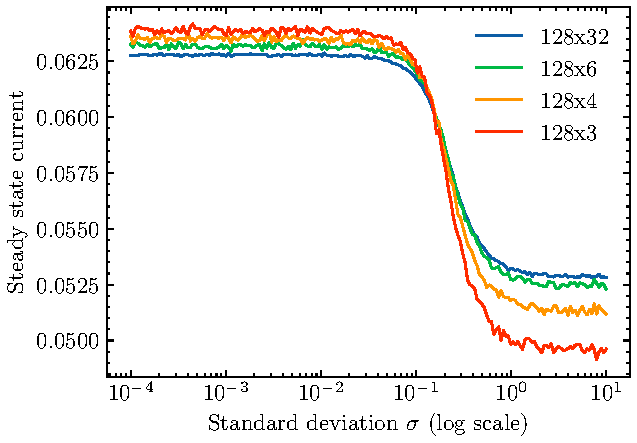
\includegraphics[width=\textwidth]{../Thesis/img/results/steady_state_current_sizes_log.pdf}
      \caption*{Steady state current as a function of $\sigma$ for different system sizes.}
    \end{figure}
  \end{columns}
\end{frame}

\begin{frame}{A Naive Policy}
  \begin{columns}
    \column{0.35\textwidth}
    \begin{block}{Just go forward?}
      \begin{itemize}
        \item $p_\text{fwd} = 1, p_\text{up/down} = 0$
        \item starting in checkerboard configuration
        \item no messy mixing
        \item bad for high $\sigma$
        \item optimum for low $\sigma$?
      \end{itemize}
    \end{block}
    \begin{align*}
      \max \left\langle J \right\rangle &= \max \left( p_\text{occ} \cdot p_\text{spd} \cdot p_\text{fwd} \cdot p_\text{emp} \right) \\
      &\le \rho \cdot \mu \cdot 1 \cdot \max(p_\text{emp}) 
    \end{align*}
    \begin{equation*}
     \text{and}\quad 0.5 \le \max(p_\text{emp}) < 1
    \end{equation*}
    \column{0.6\textwidth}
    \begin{figure}
      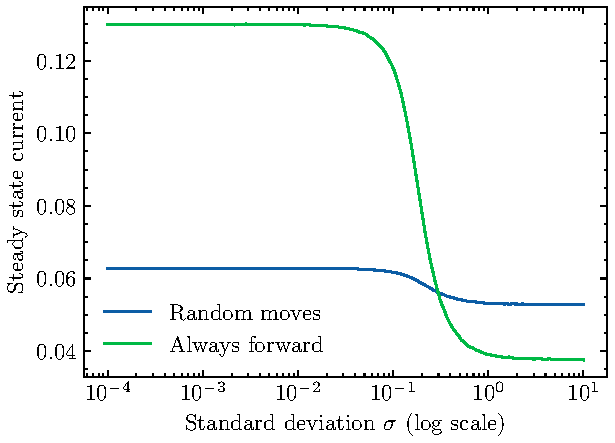
\includegraphics[width=\textwidth]{../Thesis/img/results/steady_state_current_both_log.pdf}
      \caption*{Naive policy}
    \end{figure}
  \end{columns}
  
\end{frame}

\end{document}